%!TEX root = ../notes.tex
\section{April 23, 2025}
\label{20250423}

In this lecture, we will continue our discussion of elliptic curve cryptography, and wrap up with a discussion of the practical construction of block ciphers.

\subsection{Elliptic Curve Cryptography (cont.)}

The lecture started with a brief review of elliptic curve cryptography, including a review of the chord method and tangent method to help find rational points on the curve.

Geometrically, one can be convinced that $(P \boxplus Q) \boxplus X = P \boxplus (Q\boxplus X)$ and that $P \boxplus Q = Q \boxplus P$. This gives hope that we can construct a group out of this, which is very handy for cryptography!

\begin{definition}
    For prime $p >3$, let $\mathbb{F}_p$ be a finite field, i.e. all of the integers $\{0, 1, \dots, p-1\}$ with addition and multiplication. Let $a, b \in \mathbb{F}_p$ such that $4a^3 + 27b^2 \neq 0$.
    
    An \textbf{elliptic curve $E$ defined over $\mathbb{F}_p$}, denoted $E / \mathbb{F}_p$, is the set of all points $(x,y)$ such that
    \begin{itemize}
        \item $x,y \in \mathbb{F}_p$ and
        \item $y^2 = x^3 + ax +b$
    \end{itemize}

    Additionally, we include an abstract element $\mathcal{O}$ that is thought of as the ``point at infinity''.
\end{definition}

\begin{example}
    $y^2 = x^3 + 1$ over $\mathbb{F}_{11}$ consists of the points
    $$E / \mathbb{F}_{11} = \{\mathcal{O}, (-1, 0), (0, \pm 1), (2, \pm 3), (5, \pm 4), (7, \pm 5), (9, \pm 2)\}$$
\end{example}

Elliptic curves over finite fields is the same definition as elliptic curves before except we restrict our attention to $\mathbb{F}_p$.

\begin{proposition}
    Elliptic curves over finite fields with the $\boxplus$ operation form a group.
    \begin{enumerate}
        \item \textbf{Closure:} $\forall g, h \in G, g\boxplus h \in G$. This is true because $g,h$ defines a line, and we can figure out the equation for this line over the finite field because finite fields support division. After we find the line, we can plug it into the curve equation to get a cubic equation. We have two roots, and we know the product of all of the roots is negative the constant term in the cubic equation. Since finite fields support division, we can recover the third root.
        \item \textbf{Existence of identity:} $\exists e \in G $ such that $\forall g\in G, e \boxplus g = g \boxplus e = g$. We let $e = \mathcal{O}$ be the identity. 
        \item \textbf{Existence of inverse:} $\forall g \in G, \exists h \in G, $ such that $g \boxplus h = h \boxplus g = e$. If $g = (x,y)$, then the inverse $h = (x, -y)$. You can see that drawing a line between $g,h$ gives us the point at infinity, so $g \boxplus h = \mathcal{O}$.
        \item \textbf{Associativity:} $\forall g_1, g_2, g_3 \in G, (g_1 \boxplus g_2) \boxplus g_3 = g_1 \boxplus (g_2 \boxplus g_3)$. We discussed this earlier.
        \item \textbf{Commutativity (for abelian groups):} $\forall g,h \in G, g\boxplus h = h \boxplus g.$ We discussed this earlier.
    \end{enumerate}
\end{proposition}

Furthermore, the \textbf{SEA algorithm} can count the number of points on $E / \mathbb{F}_p$ in polylog(p) time. Thus, figuring out the order of the group does not give us a problem.

Below are some curves that are standardized and used in practice. We only talk about the first one. The others are secure to use in practice and have some tradeoffs that you are welcome to look into.

\begin{itemize}
    \item curve secp2546r1 (P256) \begin{itemize}
        \item Prime $p = 2^{256} - 2^{224} + 2^{192} + 2^{96} -1$, hence only needs 256 bits to store!
        \item $y^2 = x^3 -3x + b$ for some constant $b$ that is a 255-bit string.
        \item Number of points on the curve is prime (close to p).
        \item Standardized generator point $G$. It does not have to be this particular $G$, since every point is a generator, but it is standardized so that everyone can agree on the generator to run DH key exchange for example.
    \end{itemize}
    \item curve secp256k1
    \item curve 25519
\end{itemize}


\subsection{Block Cipher}

In this course, we used block ciphers (e.g. AES), but we have not yet talked about how to construct them.

\begin{definition}
    A block cipher is a map $F: \{0, 1\} ^\lambda \times \{ 0 , 1\} ^n \to \{ 0, 1 \}^n$, where $\lambda$ is the key length and $n$ is the block length. $F_k(\cdot)$ will be a permutation/bijection from $\{0, 1\}^n$ to $\{0, 1\}^n$. $F_k^{-1}(\cdot)$ is efficiently computable given $k$.
    
    $F$ is assumed to be a \textbf{pseudorandom permutation} (PRP).
\end{definition}

\begin{example}
    \textbf{Advanced Encryption Standard (AES)} has key length $\lambda = 128, 192, \text{or }256$. The block length is $n=128$.
    
    Before AES, there was the \textbf{Data Encryption Standard (DES)} with $\lambda = 56$ and $n =64$.
\end{example}

We will see how to construct DES, which has similar ideas in constructing AES. To do so, we need to talk about Substitution-Permutation Networks (SPN) and Feistel Networks.

\subsection{Substitution-Permutation Network (SPN)}

We want to incorporate a design principle known as the ``Avalanche Effect'', where a small change in the input should have an effect on every part of the output. In particular, even if one-bit is changed in the input, every bit in the output should be affected so that it looks completely different.

SPN proceeds as follows.

\begin{enumerate}
    \item[Step 1.] \textbf{Key mixing.} Take input $x$ and XOR it with sub-key $k$, i.e. $x:= x \oplus k$. The result is 64-bit.
    \item[Step 2.] \textbf{Confusion Step.} Split $x$ into $8$ parts of 8 bits each. On each part, apply an \textbf{S-box}, which is a public permutation of 8 bits. Furthermore, 1-bit change in the input gives a 2-bit change in the output.
    \item[Step 3.] \textbf{Diffusion Step.} Take the output from each S-box and concatenate them together into a 64-bit result. Then use a public mixing permutation to shuffle the bits.
\end{enumerate}

\begin{center}
    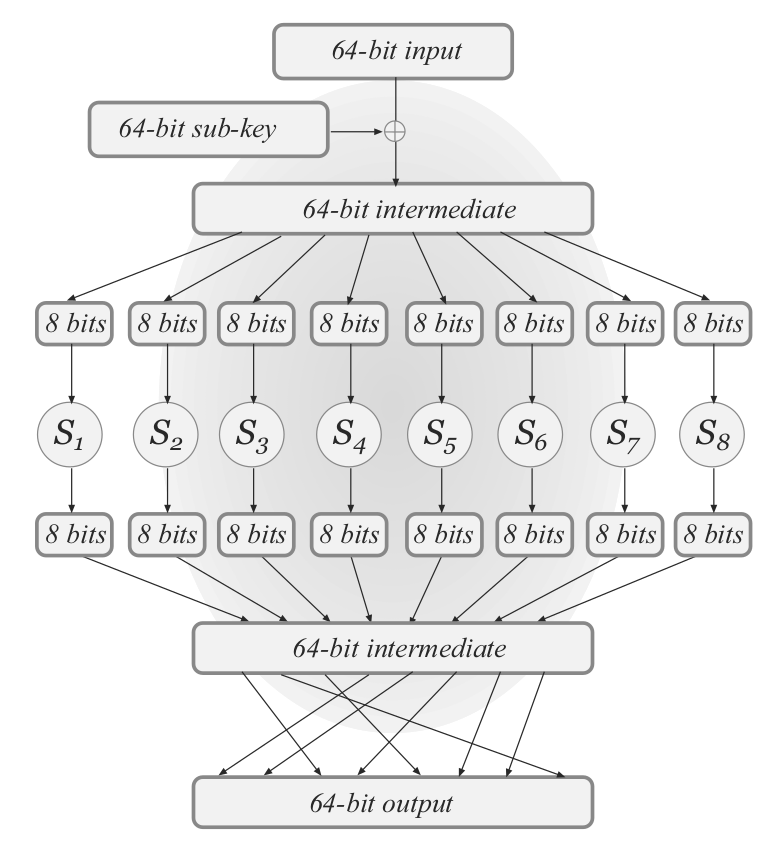
\includegraphics[width=0.5\linewidth]{2024-04-15-spn.png}
\end{center}

We can repeat this procedure for multiple rounds. For example, below is a 3-round SPN.

\begin{center}
    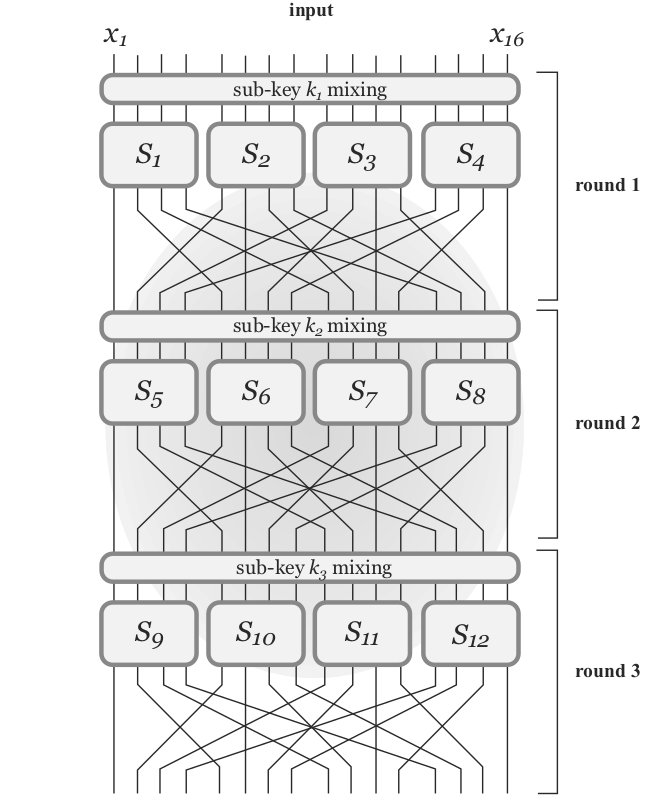
\includegraphics[width=0.5\linewidth]{2024-04-15-spn-mult.png}
\end{center}

Different sub-keys are used in each round. These sub-keys are derived from a \textit{master key} using a \textit{key schedule}, for example, by taking different subsets from the master key.

Given the master key, we can compute $F_{k}^{-1}(y)$. First, use the key schedule to find each sub-key, which we can use to XOR to get the inverse. Then, since each mixing permutation is public, we can compute its inverse for each round. Additionally, each S-box is public, so we can find its inverse too. Thus we have all the information we need to compute the inverse.

\subsection{Attacks on Reduced-Round SPN}

\textbf{1-round SPN without final key mixing.} The adversary can begin with the output $y$, then invert it starting from the end to the beginning. Since the permutations are public, the adversary can compute $x \oplus k$, and since they know the input $x$, they can figure out $k$. Thus we have a complete break. This shows that we need a final key mixing step.

\textbf{1-round SPN with final key mixing.} Assume the key and input is 16-bit. The adversary can try to attack by enumerate the possible values of $k_2$, then using the SPN derive $k_1$ for each $k_2$. This takes $O(2^{16})$ time and gives $2^{16}$ possible values for the master key.

\subsection{Feistel Network}

\begin{center}
    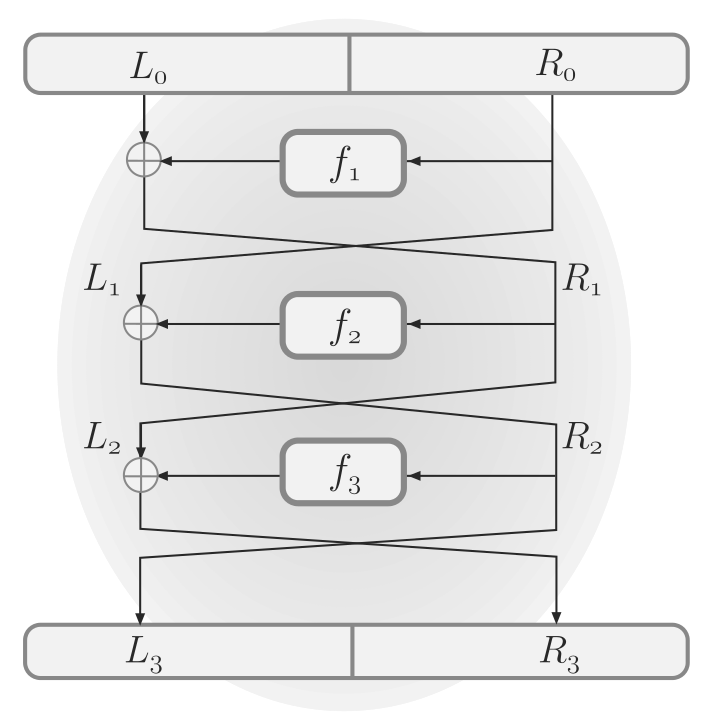
\includegraphics[width=0.5\linewidth]{2024-04-15-feistel-3round.png}
\end{center}

Let $x = L_0 || R_0$ be the input split into two halves, left and right. The $R_0$ is fed into a \textit{round function} $f_1$ and is XOR-ed with $L_0$ to get $R_1$. Then $L_1$ is defined to be $R_0$. This is repeated for several rounds (3 rounds in the figure above). Let $y= L_n || R_n$ be the output after $n$ rounds.

To compute the inverse $F_k^{-1}(y)$, start from the output e.g. $(L_3, R_3)$. We know $R_2 = L_3$, so we can compute $f_3(R_2)$. This satisfies $f_3(R_2) \oplus L_2 = R_3$, so we can find $L_2$. Thus we have found $(L_2, R_2)$, and we can continue until we get $x$.

There are attacks on reduced-round Feistel Networks that we will not cover in lecture, but you can think about it on your own.

\subsection{Data Encryption Standard (DES)}

Recall that the block length is $n=64$ and master key length is $\lambda = 56$ for DES. Use the Feistel network on our $64$-bit input $x$ so that $L_0, R_0$ each get $32$ bits. For the round functions, we use something called a \textit{DES mangler function}, which is essentially a SPN.

However, unlike an SPN, the S-boxes are not permutation, but rather they reduce the size from 6-bit to 4-bit. Additionally, the follow the following properties
\begin{enumerate}
    \item Maps $\{0, 1\}^6 \to \{0, 1\}^4$.
    \item ``4-to-1'': Exactly 4 inputs map to the same output.
    \item 1-bit change of input gives at least 2-bit change in the output.
\end{enumerate}

\begin{center}
    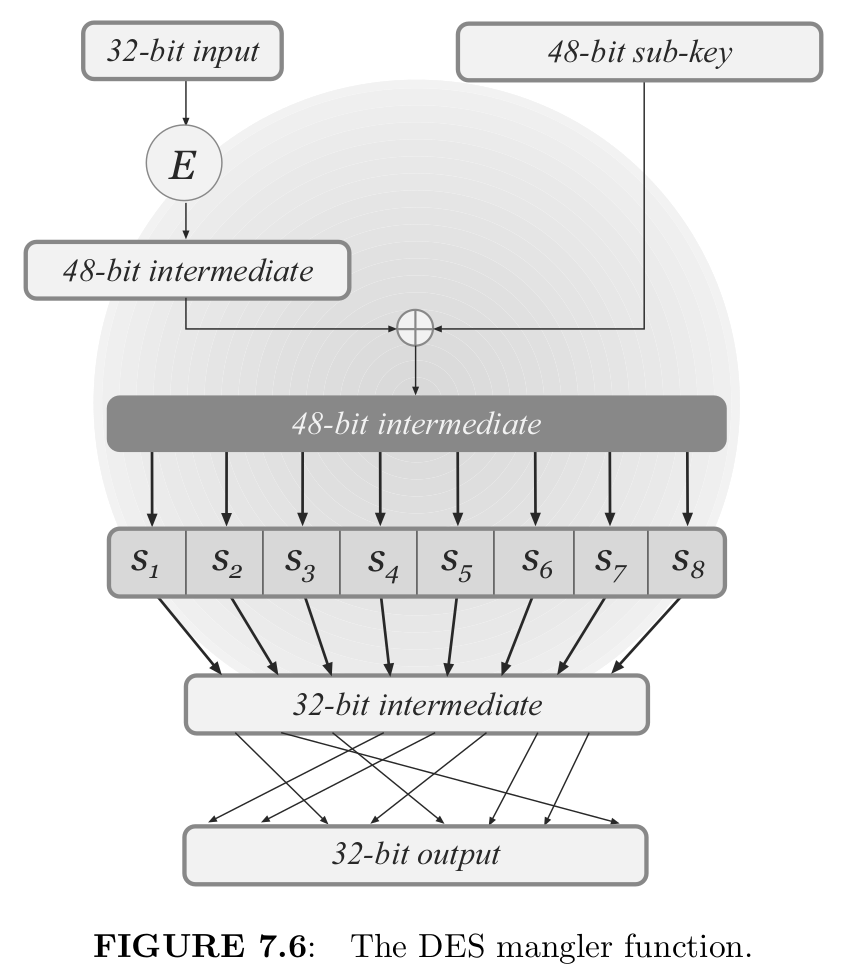
\includegraphics[width=0.5\linewidth]{2024-04-15-dsa-mangler.png}
\end{center}

$E$ is an expansion function. Given a 32-bit string AB where A and B are 16-bit, the output is a 42-bit string ABA.

For the key schedule, we have a master key with length 56 but need a 48-bit sub-key. To do so, split the master key into two halves of 28-bits each, then take a random subset of 24-bits from each half. Then concatenate these two subsets to form a 48-bit sub-key.

\begin{remark}
    DES does seem very complicated. This is intentional to do so so that attacks are hard.

    Multiple rounds of DES does not necessarily improve the security guarantees. Once DES is applied multiple times, we lose our security guarantee, and we need to do additional cryptanalysis, so it is unclear if it is secure. This is the reason NIST developed a new standard known as AES.
\end{remark}

